\begingroup \renewcommand{\arraystretch}{1}
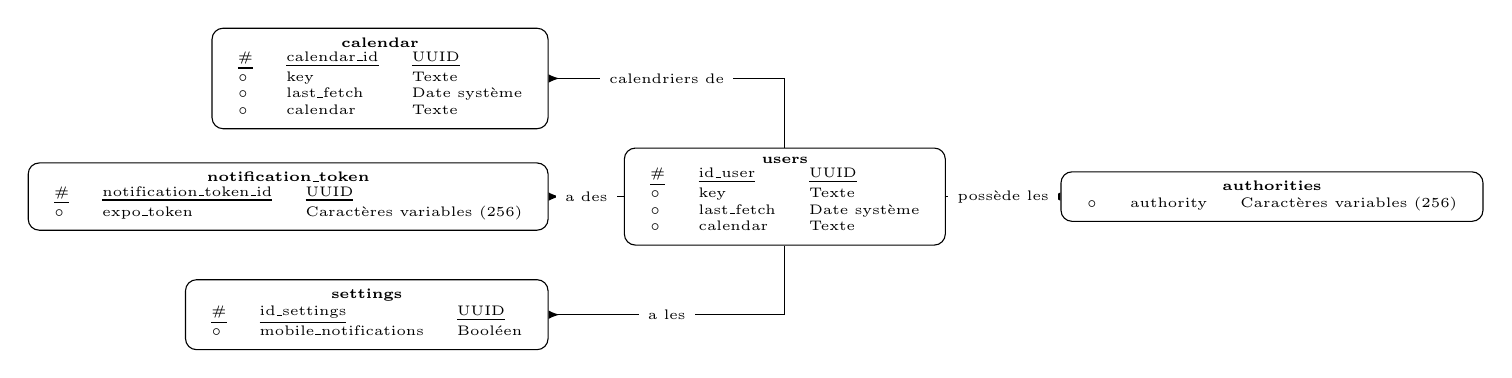
\begin{tikzpicture}\tikzstyle{every node}=[font=\tiny]
% users
  \node[draw, rounded corners, align=center] (users) at (0,0)%
{%
  \bf users \\
  \begin{tabular}{lll}
    \underline{\#} & \underline{id\_user} & \underline{UUID} \\
    $\circ$ & key & Texte \\
    $\circ$ & last\_fetch & Date système \\
    $\circ$ & calendar & Texte
  \end{tabular}
};
% calendar
  \node[draw, rounded corners, align=center, anchor=east] (cal) at (-3,1.5)%
{%
  \bf calendar \\
  \begin{tabular}{lll}
    \underline{\#} & \underline{calendar\_id} & \underline{UUID} \\
    $\circ$ & key & Texte \\
    $\circ$ & last\_fetch & Date système \\
    $\circ$ & calendar & Texte
  \end{tabular}
};
% notification_token
  \node[draw, rounded corners, align=center, anchor=east] (notif) at (-3,0)%
{%
  \bf notification\_token \\
  \begin{tabular}{lll}
    \underline{\#} & \underline{notification\_token\_id} & \underline{UUID} \\
    $\circ$ & expo\_token & Caractères variables (256)
  \end{tabular}
};
% settings
  \node[draw, rounded corners, align=center, anchor=east] (settings) at (-3,-1.5)%
{%
  \bf settings \\
  \begin{tabular}{lll}
    \underline{\#} & \underline{id\_settings} & \underline{UUID} \\
    $\circ$ & mobile\_notifications & Booléen
  \end{tabular}
};
% authorities
  \node[draw, rounded corners, align=center, anchor=west] (auth) at (3.5,0)%
{%
  \bf authorities \\
  \begin{tabular}{lll}
    $\circ$ & authority & Caractères variables (256)
  \end{tabular}
};
%%%%%%%%%%%%%%%%
\draw[-latex reversed] (users.west) -- node[midway, fill=white] {a des} (notif.east);
\draw[-latex reversed] (users.south) -- (0,-1.5) -- node[midway, fill=white] {a les}(settings.east);
\draw[-latex reversed] (users.north) -- (0,1.5) -- node[midway, fill=white] {calendriers de} (cal.east);
\draw[-latex reversed] (users.east) -- node[midway, fill=white] {possède les}(auth.west);
\end{tikzpicture}
\endgroup